\section{Sucesiones y series de funciones}

\subsection{Sucesiones de funciones. Convergencia y tipos de convergencia}

\begin{nota}
    En lo sucesivo sea $D \subseteq \R$, entonces
    
    \[
    A(D) = \{f: D \rightarrow \R : f \text{ es acotada}\}
    \]
    
    Sabemos que se cumple lo siguiente:
    
    \begin{itemize}
        \item $f,g \in A(D)$ entonces $f+g \in A(D)$.
        \item $\lambda \in \R$, $f \in A(D)$ entonces $\lambda f \in A(D)$.
    \end{itemize}
    
    Luego $A(D)$ es un espacio vectorial. Dotemos a este conjunto con una norma:
    
    \[
    \norma{f} = \sup_{x \in D} |f (x)|
    \]
    
    Sean $f,g \in A(D)$ y $\lambda \in \R$. Esta norma cumple con las siguientes propiedades\marginfootnote{
    \begin{ejer}
        Demostrar estas propiedades.
    \end{ejer}}:
    
    \begin{itemize}
        \item $\norma{f} = 0$ sii $f \equiv 0$.
        \item $\norma{\lambda f} = |\lambda|\norma{f}$.
        \item $\norma{f + g} \leq \norma{f} + \norma{g}$.
    \end{itemize}
    
    En conclusión, $(A(D), \norma{\dots})$ es un espacio vectorial normado.
\end{nota}

Bajo este contexto, podremos desarrollar las ideas que presentaremos a continuación.

\begin{defn}
    Una \ul{sucesión} $(f_n)_{n=1}^{\infty} \in A(D)$ es una aplicación de $\N$ en $A(D)$ tal que a cada $n \in \N$ le asociamos $f_n \in A(D)$.
    
    Decimos que la sucesión \ul{converge puntualmente (c.p)} si dado $x \in D$ tenemos que
    
    \[
    \limtoinfty{n}{f(x)} = f(x)
    \]
    
    \noindent es decir, existe una función $f$ tal que para cada $x \in D$, $f$ es el límite de la sucesión. En términos $\varepsilon$, $\delta$ podemos definir la convergencia puntual de la siguiente manera: Dados $\varepsilon > 0$ y $x \in D$, existe un $N_{\varepsilon} \in \N$ tal que $|f_n(x) - f(x)| < \varepsilon$ si $n \geq N_{\varepsilon}$.
\end{defn}

\begin{ejem}\label{ejem:cp}
    Consideremos los siguientes ejemplos para afianzar la definición:
    
    \begin{enumerate}
        \item Sea $D = [0,1]$, y la sucesión $f_n(x) = x^n$. ¿Qué sucede con el límite cuando $n \rightarrow \infty$. Primero, grafiquemos la sucesión:
        
        \begin{figure}
            \centering
            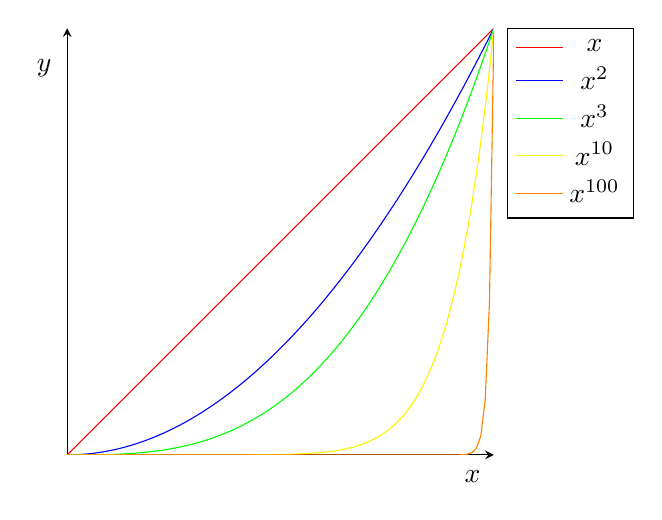
\begin{tikzpicture}
                \begin{axis}[
                    axis x line = bottom,
                    axis y line = left,
                    domain=0:1,
                    width=7cm,
                    height=7cm,
                    xtick=\empty,
                    ytick=\empty,
                    every axis x label/.style={at={(ticklabel cs: 0.95,0)},
                    anchor=north},
                    every axis y label/.style={at={(ticklabel cs: 0.95,0)},
                    anchor=north east},
                    xlabel=$x$,
                    ylabel=$y$,
                    legend cell align=center,
                    legend pos=outer north east
                    ]
                    \addplot[red,samples=100] {x};
                    \addplot[blue,samples=100] {x^2};
                    \addplot[green,samples=100] {x^3};
                    \addplot[yellow,samples=100] {x^10};
                    \addplot[orange,samples=100] {x^100};
                    \legend{$x$,$x^2$,$x^3$, $x^{10}$, $x^{100}$};
                \end{axis}
            \end{tikzpicture}
            \label{fig:ej4.1}
            \caption{\footnotesize Gráfica para la sucesión $f_n(x) = x^n$. Vemos que la sucesión cada vez se acerca más al eje $x$.}
        \end{figure}
        
        Vemos que todas las funciones pasan por $0$ y pasan por $1$, entonces no importa cuál sea el valor de $n$, todas pasan por estos valores. El estudio de estas gráficas consecutivas, nos permite deducir que al tomar $n \rightarrow \infty$ tendremos que\marginfootnote{Recordemos que, $\limtoinfty{n}{x^n} = 0$ sii $|x|<1$. Este es un resultado que se estudió al revisar las sucesiones numéricas.}
        
        \[
        \limtoinfty{n}{f_n(x)} = f(x), \quad \text{donde} \quad f(x)=\begin{cases}
        0 \quad \text{si} \quad x \in [0,1) \\
        1 \quad \text{si} \quad x = 1
        \end{cases}
        \]
        
        \item Sea la sucesión
        
        \[
        f_{n-1}(x) =
        \begin{cases}
            0& x \in \left[0, \frac{1}{n}\right] \cup \left[\frac{2}{n}, 1\right] \\
            2n& x \in \left(\frac{1}{n}, \frac{2}{n}\right)
        \end{cases}
        \]
        
        Grafiquemos la función para varios casos de $n$:
        
        \begin{figure}
            \begin{subfigure}[b]{.5\textwidth}
                \centering
                \begin{tikzpicture}
                    \begin{axis}[
                        axis x line = bottom,
                        axis y line = left,
                        domain=0:1,
                        width=5cm,
                        height=5cm,
                        xtick={0,1/2},
                        ytick=\empty,
                        every axis x label/.style={at={(ticklabel cs: 0.95,0)},
                        anchor=south},
                        every axis y label/.style={at={(ticklabel cs: 0.95,0)},
                        anchor=north east},
                        xlabel=$x$,
                        ylabel=$y$,
                        legend cell align=center,
                        legend pos=outer north east
                        ]
                        \addplot[red,samples=100,domain=1/2:1] {4};
                        \addplot[blue,samples=100,domain=0:1/2] {0};
                        \legend{$4$};
                    \end{axis}
                \end{tikzpicture}
                \caption{\footnotesize Gráfica para $n=1$.}
            \end{subfigure}
            \hfill
            \begin{subfigure}[b]{.5\textwidth}
                \centering
                \begin{tikzpicture}
                    \begin{axis}[
                        axis x line = bottom,
                        axis y line = left,
                        domain=0:1,
                        width=5cm,
                        height=5cm,
                        xtick={0,1/3,2/3},
                        ytick=\empty,
                        every axis x label/.style={at={(ticklabel cs: 0.95,0)},
                        anchor=south},
                        every axis y label/.style={at={(ticklabel cs: 0.95,0)},
                        anchor=north east},
                        every plot/.append style={very thick},
                        xlabel=$x$,
                        ylabel=$y$,
                        legend cell align=center,
                        legend pos=outer north east
                        ]
                        \addplot[red,samples=100,domain=1/3:2/3] {6};
                        \addplot[blue,samples=100,domain=0:1/3] {0};
                        \addplot[blue,samples=100,domain=2/3:1] {0};
                        \node[fill,circle,color=red,inner sep=1.5pt] at
(920,590){};
                        \legend{6};
                    \end{axis}
                \end{tikzpicture}
                \caption{\footnotesize Gráfica para $n=2$.}
            \end{subfigure}
            \hfill
            \vfill
            \begin{subfigure}[b]{.5\textwidth}
            \centering
                \begin{tikzpicture}
                    \begin{axis}[
                        axis x line = bottom,
                        axis y line = left,
                        domain=0:1,
                        width=5cm,
                        height=5cm,
                        xtick={0,1/4,1/2},
                        ytick=\empty,
                        every axis x label/.style={at={(ticklabel cs: 0.95,0)},
                        anchor=south},
                        every axis y label/.style={at={(ticklabel cs: 0.95,0)},
                        anchor=north east},
                        every plot/.append style={very thick},
                        xlabel=$x$,
                        ylabel=$y$,
                        legend cell align=center,
                        legend pos=outer north east
                        ]
                        \addplot[red,samples=100,domain=1/4:1/2] {8};
                        \addplot[blue,samples=100,domain=0:1/4] {0};
                        \addplot[blue,samples=100,domain=1/2:1] {0};
                        \node[fill,circle,color=red,inner sep=1.5pt] at
(920,780){};
                        \legend{8};
                    \end{axis}
                \end{tikzpicture}
                \caption{\footnotesize Gráfica para $n=3$.}
            \end{subfigure}
            \hfill
            \begin{subfigure}[b]{.5\textwidth}
            \centering
                \begin{tikzpicture}
                    \begin{axis}[
                        axis x line = bottom,
                        axis y line = left,
                        domain=0:1,
                        width=5cm,
                        height=5cm,
                        xtick={0,1/5,2/5},
                        ytick=\empty,
                        every axis x label/.style={at={(ticklabel cs: 0.95,0)},
                        anchor=south},
                        every axis y label/.style={at={(ticklabel cs: 0.95,0)},
                        anchor=north east},
                        every plot/.append style={very thick},
                        xlabel=$x$,
                        ylabel=$y$,
                        legend cell align=center,
                        legend pos=outer north east
                        ]
                        \addplot[red,samples=100,domain=1/5:2/5] {10};
                        \addplot[blue,samples=100,domain=0:1/5] {0};
                        \addplot[blue,samples=100,domain=2/5:1] {0};
                        \node[fill,circle,color=red,inner sep=1.5pt] at
(920,98.2){};
                        \legend{10};
                    \end{axis}
                \end{tikzpicture}
                \caption{\footnotesize Gráfica para $n=4$.}
            \end{subfigure}
            \caption{\footnotesize Gráfica de $f_{n}$ definida como en el segundo ejemplo para varios valores de $n$.}
            \label{fig:ej4.2}
        \end{figure}
        
        Vemos que a medida que $n$ crece, las rectas que no son $0$, cada vez se van achicando y van tomando valores más grandes para $y$. Entonces, si $n \rightarrow \infty$, $\left[0, \frac{1}{n}\right] \cup \left[\frac{2}{n}, 1\right] \rightarrow [0,1]$, y por la misma razón, $\left(\frac{1}{n}, \frac{2}{n}\right) \rightarrow \emptyset$. Entonces,
        
        \[
        \limtoinfty{n}{f_n(x)} = f(x)
        \]
        
        donde $f(x) = 0$, $\forall x \in [0,1]$.
    \end{enumerate}
\end{ejem}

\begin{defn}
    Dada una sucesión $(f_n)_{n=1}^{\infty} \in A(D)$ definimos las \ul{sumas parciales} como
    
    \[
    S_N(x) = f_1(x) + \dots + f_N(x)
    \]
    
    \noindent para cada $x \in D$.
    
    La serie $\sum_{k=1}^{\infty} f_k(x)$ \ul{converge} para cada $x \in D$ si $\limtoinfty{N}{S_N(x)}$ existe para cada $x \in D$.
\end{defn}

\begin{ejem}
    Consideremos $f_n(x)$ definida como
    
    \[
    f_n(x)=\begin{cases}
        0& \quad \left[0, \frac{1}{n+1}\right) \cup \left(\frac{1}{n}, 1\right) \\
        1& \quad \left(\frac{1}{n+1}, \frac{1}{n}\right] \cup \{1\}
    \end{cases}
    \]
    
    Entonces, ¿$\sum_{n=1}^{\infty} f_n(x)$ converge puntualmente? Grafiquemos esta función:
    
    \vspace{5mm}
    
        \begin{figure}
            \begin{subfigure}[b]{.5\textwidth}
                \centering
                \begin{tikzpicture}
                    \begin{axis}[
                        axis x line = bottom,
                        axis y line = left,
                        domain=0:1,
                        width=5cm,
                        height=5cm,
                        xtick={0,1/2},
                        ytick=\empty,
                        every axis x label/.style={at={(ticklabel cs: 0.95,0)},
                        anchor=south},
                        every axis y label/.style={at={(ticklabel cs: 0.95,0)},
                        anchor=north east},
                        every plot/.append style={very thick},
                        xlabel=$x$,
                        ylabel=$y$,
                        legend cell align=center,
                        legend pos=outer north east
                        ]
                        \addplot[red,samples=100,domain=1/2:1] {1};
                        \addplot[blue,samples=100,domain=0:1/2] {0};
                        \legend{$1$};
                    \end{axis}
                \end{tikzpicture}
                \caption{\footnotesize Gráfica para $n=1$.}
            \end{subfigure}
            \hfill
            \begin{subfigure}[b]{.5\textwidth}
                \centering
                \begin{tikzpicture}
                    \begin{axis}[
                        axis x line = bottom,
                        axis y line = left,
                        domain=0:1,
                        width=5cm,
                        height=5cm,
                        xtick={0,1/3,1/2,2/3},
                        ytick=\empty,
                        every axis x label/.style={at={(ticklabel cs: 0.95,0)},
                        anchor=south},
                        every axis y label/.style={at={(ticklabel cs: 0.95,0)},
                        anchor=north east},
                        every plot/.append style={very thick},
                        xlabel=$x$,
                        ylabel=$y$,
                        legend cell align=center,
                        legend pos=outer north east
                        ]
                        \addplot[red,samples=100,domain=1/3:1/2] {1};
                        \addplot[blue,samples=100,domain=0:1/3] {0};
                        \addplot[blue,samples=100,domain=1/2:1] {0};
                        \node[fill,circle,color=red,inner sep=1.5pt] at
(920,98.2){};
                        \legend{1};
                    \end{axis}
                \end{tikzpicture}
                \caption{\footnotesize Gráfica para $n=2$.}
            \end{subfigure}
            \hfill
            \vfill
            \begin{subfigure}[b]{.5\textwidth}
            \centering
                \begin{tikzpicture}
                    \begin{axis}[
                        axis x line = bottom,
                        axis y line = left,
                        domain=0:1,
                        width=5cm,
                        height=5cm,
                        xtick=\empty,
                        ytick=\empty,
                        every axis x label/.style={at={(ticklabel cs: 0.95,0)},
                        anchor=south},
                        every axis y label/.style={at={(ticklabel cs: 0.95,0)},
                        anchor=north east},
                        every plot/.append style={very thick},
                        xlabel=$x$,
                        ylabel=$y$,
                        legend cell align=center,
                        legend pos=outer north east
                        ]
                        \addplot[red,samples=100,domain=1/3:1/4] {1};
                        \addplot[blue,samples=100,domain=0:1/4] {0};
                        \addplot[blue,samples=100,domain=1/3:1] {0};
                        \node[fill,circle,color=red,inner sep=1.5pt] at
(920,98.2){};
                        \legend{1};
                    \end{axis}
                \end{tikzpicture}
                \caption{\footnotesize Gráfica para $n=3$.}
            \end{subfigure}
            \hfill
            \begin{subfigure}[b]{.5\textwidth}
            \centering
                \begin{tikzpicture}
                    \begin{axis}[
                        axis x line = bottom,
                        axis y line = left,
                        domain=0:1,
                        width=5cm,
                        height=5cm,
                        xtick=\empty,
                        ytick=\empty,
                        every axis x label/.style={at={(ticklabel cs: 0.95,0)},
                        anchor=south},
                        every axis y label/.style={at={(ticklabel cs: 0.95,0)},
                        anchor=north east},
                        every plot/.append style={very thick},
                        xlabel=$x$,
                        ylabel=$y$,
                        legend cell align=center,
                        legend pos=outer north east
                        ]
                        \addplot[red,samples=100,domain=1/4:1/5] {1};
                        \addplot[blue,samples=100,domain=0:1/5] {0};
                        \addplot[blue,samples=100,domain=1/4:1] {0};
                        \legend{1};
                    \node[fill,circle,color=red,inner sep=1.5pt] at
(920,98.2){};
                    \end{axis}
                \end{tikzpicture}
                \caption{\footnotesize Gráfica para $n=4$.}
            \end{subfigure}
            \caption{\footnotesize Gráfica de $f_{n}$ definida como en el ejemplo para varios valores de $n$.}
            \label{fig:ej4.2}
        \end{figure}
        
    Luego, tenemos
    
    \begin{itemize}
        \item $\displaystyle S_1(x) = f_1(x) =\begin{cases}
            0& \quad x \in \left[0,\frac{1}{2}\right) \\
            1& \quad x \in \left[\frac{1}{2}, 1\right]
        \end{cases}$.
        \item $\displaystyle S_2(x) = f_1(x) + f_2(x) =\begin{cases}
            0& \quad x \in \left[0,\frac{1}{3}\right) \\
            1& \quad x \in \left[\frac{1}{3}, 1\right]
        \end{cases}$.
        \item $\displaystyle S_3(x) = S_2(x) + f_3(x) =\begin{cases}
            0& \quad x \in \left[0,\frac{1}{4}\right) \\
            1& \quad x \in \left[\frac{1}{4}, 1\right]
        \end{cases}$.
        \item $\displaystyle S_4(x) = S_3(x) + f_4(x) =\begin{cases}
            0& \quad x \in \left[0,\frac{1}{5}\right) \\
            1& \quad x \in \left[\frac{1}{5}, 1\right]
        \end{cases}$.
    \end{itemize}
    
    Al hacer esto de forma sucesiva, tendremos
    
    \[
    \limtoinfty{N}{S_N(x)} = f(x) \quad \text{donde $f(x) = 1$}
    \]
    
    \noindent y esto $\forall x \in [0,1]$.
    
    En conclusión,
    
    \[
    \sum_{n=1}^{\infty} f_n(x) = 1 \quad \forall x \in [0,1]
    \]
\end{ejem}

Pero en líneas generales, calcular la convergencia no es un asunto tan trivial. Veamos ahora otro ejemplo un poco más breve que el anterior:

\begin{ejem}\label{ej:x^n}
    Sea $f_n(x) = x^n$ con $n\geq0$ y $x \in [0,1]$, entonces $S_N(x) = 1 + \dots + x^n$. Por propiedades de polinomios, tendremos que
    
    \[
    S_N(x) = \frac{1-x^{N+1}}{1-x}
    \]
    
    Ahora, sabemos que
    
    \[
    \limtoinfty{N}{x^N} = 0 \iff |x| < 1
    \]
    
    Utilizando este resultado, tendremos que
    
    \[
    \limtoinfty{N}{\frac{1 - x^{N+1}}{1-x}}  = \frac{1}{1-x} \quad \text{para cada $x \in [0,1]$}
    \]
    
    De esta manera, $\limtoinfty{N}{S_N(x)} = \frac{1}{1-x}$. En consecuencia,
    
    \[
    \sum_{N=0}^{\infty} x^N = \frac{1}{1-x} \quad \forall x \in [0,1]
    \]
\end{ejem}

\begin{defn}
    Sea $\left(f_n\right)_{n=1}^{\infty} \in A(D)$, diremos que $\limtoinfty{n}{f_n} = f$ \ul{uniformemente (c.u)} \marginfootnote{Tanto en el Spivak como en el Apostol se da una definición distinta de convergencia uniforme, pero que es equivalente. Un buen ejercicio es demostrar la equivalencia de ambas definiciones.} si
    
    \[
    \limtoinfty{n}{\norma{f_n - f}} = 0
    \]
    
    Esto equivale a: Dado $\varepsilon > 0$. $\exists N_{\varepsilon} \in \N$ tal que
    
    \[
    \text{si} \quad n \geq N_{\varepsilon} \implies \norma{f_n - f} < \varepsilon
    \]
\end{defn}

Lo que estudiaremos a continuación es la relación entre la convergencia puntual y la convergencia uniforme.

\begin{pro}
    Sea $\left(f_n\right)_{n=1}^{\infty} \in A(D)$. Si $\sucinf{f}{n}$ c.u a $f$, entonces $\sucinf{f}{n}$ c.p a $f$.
\end{pro}

\begin{proof}
    Consideremos $\varepsilon > 0$. Entonces existe un $N_{\varepsilon} \in \N$ tal que si $n \geq N_{\varepsilon}$ entonces
    
    \[
    \norma{f_n - f} < \varepsilon
    \]
    
    Como $\norma{f_n - f} = \sup_{x \in D} \left| f_n(x) - f(x) \right| \geq |f_n(x) - f(x)|$, entonces nos queda que
    
    \[
    |f_n(x) - f(x)| < \epsilon
    \]
    
    En conclusión, dado $\varepsilon > 0$ si $n \geq N_{\varepsilon}$ entonces $|f_n(x) - f(x)| < \epsilon$ para $x \in D$. Esta es la definición de convergencia puntual, por lo que queda demostrado.
\end{proof}

\begin{nota}
    Al igual que antes, en lo sucesivo consideremos
    
    \[
    C(D) = \{f: D \rightarrow \R : \text{$f$ es continua}\}
    \]
\end{nota}

\begin{ejem}
    Sea $f_n(x) = x^n$, con $n \geq 0$ y $D = [0,1]$. Como todas estas funciones son continuas, tendremos que $\sucinf{f}{n} \in C(D)$. Pero no sólo son continuas, ademas son acotadas\marginfootnote{Recordar que toda función continua, definida sobre un compacto es acotada.}.
    
    Habíamos visto anteriormente en el ejemplo \ref{ejem:cp} que el límite puntual nos dió como resultado
    
    \[
    f(x) = \begin{cases}
        0& x \in [0,1)] \\
        1& x = 1
    \end{cases}
    \]
    
    \noindent pero $\limtoinfty{n}{f_n(x)} = f(x) \notin C[0,1]$\marginfootnote{Esta función presenta una discontinuidad de salto por la izquierda en $x=1$}.
    
    Por otro lado,
    
    \[
    \limtoinfty{n}{\norma{f_n - f}} = \limtoinfty{n}{\sup_{x \in [0,1]} \left|f_n(x) - f\right|} \neq 0
    \]
    
    \noindent por lo tanto, $\sucinf{f}{n}$ no c.u.
\end{ejem}

Con el ejemplo anterior, vemos que si tomamos una sucesión de funciones $\sucinf{f}{n} \in C(D)$, la función $f$ a la que c.p no necesariamente tiene que estar en $C(D)$. Dicho de otra forma, $C(D)$ no es cerrado bajo convergencia puntuales. Es en ese sentido que la convergencia puntual es más débil.

\begin{pro}
    Sea $\sucinf{f}{n} \in A(D)$. Si $\limtoinfty{n}{f_n} = f$ uniformemente entonces $f \in A(D)$.
\end{pro}

\begin{proof}
    Para cada $f_n \in A(D)$, $\exists M_n > 0$ tal que
    
    \begin{equation}\label{eq:cl7.1}
        |f_n(x)| \leq M_n \quad \forall x \in D
    \end{equation}
    
    Ahora, como tenemos c.u: Dado $\varepsilon > 0$, existe un $N_{\varepsilon}$ tal que
    
    \begin{equation}\label{eq:cl7.2}
        \text{si} \quad n \geq N_{\varepsilon} \implies \norma{f_n - f} < \varepsilon
    \end{equation}
    
    Por otro lado,
    
    \[
    \norma{f} = \norma{f - f_n + f_n} \leq \norma{f - f_n} + \norma{f_n}
    \]
    
    Ya que hemos elegido $N_{\varepsilon}$ tal que $n \geq N_{\varepsilon}$, entonces por \ref{eq:cl7.1} y \ref{eq:cl7.2} nos queda
    
    \[
    \norma{f} = \norma{f - f_n} + \norma{f_n} \leq \varepsilon + M_n \quad \forall n \geq N_{\varepsilon}
    \]
    
    De esta forma $\norma{f} = \sup_{x \in D} |f(x)| < \varepsilon + M_n$, en particular $\norma{f} < \varepsilon + M_{N_{\varepsilon}}$ por lo tanto $f \in A(D)$. Así queda demostrado.
\end{proof}

Luego, podemos decir que el espacio $\left(A(D), \norma{\dots} \right)$ cumple con la propiedad de completitud, es decir es cerrado desde el punto de vista topológico.